
\chapter{Grundlagen}\label{chap:grundlagen}

Die \gls{stg} beschreibt eine abstrakte Maschine, sowie eine kleine Programmiersprache zur Programmierung ebendieser Maschine, die als STG-Sprache bezeichnet wird.
Der vorwiegende Verwendungszweck liegt dabei in der Übersetzung und Ausführung von nicht-strikten funktionalen Programmiersprachen.
In solchen Programmiersprachen werden Ausdrücke verzögert und nur bei Bedarf ausgewertet.
Man spricht auch von der sogenannten \textit{Bedarfsauswertung} oder aus dem Englischen \textit{lazy Evaluation}.

Dieser Ausführungsmodus kommt mit einer Reihe an großen Herausforderungen.
Zur Laufzeit muss zwischen ausstehenden oder unterbrochenen Auswertungen (sogenannten \textit{Thunks}) und bereits berechneten Werten unterschieden werden.
Gleichzeitig soll überflüssige Arbeit vermieden werden, indem Ausdrücke nur so oft wie nötig ausgewertet werden, um anschließend deren Wert für den Falle erneuter Auswertung zu speichern.
Zudem ist es in funktionalen Sprachen häufig der Fall, dass Ausdrücke nicht nur einfache Werte sondern auch Funktionen berechnen, welche dann auf Argumente angewandt, an andere Funktionen übergeben oder an Namen gebunden werden können.
Selbstverständlich soll eine Ausführungsumgebung, die all diese Anforderungen unterstützt, auch noch möglichst effizient sein und mit möglichst wenig Speicherbedarf und Rechenzeit auskommen.

Die STG-Maschine verspricht, als abstrakte Maschine diesen Anforderungen nachzukommen und wird seit ???\cn{Datum herausfinden} als  wesentlicher Bestandteil in der Implementierung und Übersetzung von Haskell verwendet.
Im Ergebnis ist Performance von übersetzten Haskell Programmen häufig vergleichbar mit C.\cn{}


\section{Graphenreduktion als Ausführungsmodell}

Die Verwendung einer abstrakten Maschine zur Ausführung einer Programmiersprache ist keine Besonderheit.
Die ursprünglich für Java entwickelte \gls{jvm} beschreibt eine abstrakte Stackmaschine, die entweder im Rahmen einer virtuellen Maschinenimplementierung ausgeführt wird, oder deren Semantik in Maschinencode für eine reale Maschine übersetzt wird.
Um die .NET Plattform herum entstand die \gls{cli}, welche standardisiert eine objektorientierte abstrakte Stackmaschine beschreibt.
In beiden Fällen soll die Verwendung einer abstrakten Maschine über die Tatsächliche Ausführungsumgebung abstrahieren, um so Programme plattform- und hardwareunabhängig ausführen zu können.
Eine ähnliche Architektur bietet LLVM mit einer abstrakten Registermaschine.
Hier liegt der Fokus jedoch auf der Optimierung und Übersetzung von Programmen für diese abstrakte Maschine in realen Maschinencode.

All diese Modelle sind nah an dem Modell der handelsüblichen Computer, welche auch als sogenannte Sequentielle Maschinen~\cite{Slot_ProblemSpaceInvariance} Einzug in die theoretische Welt der Berechenbarkeit gehalten haben.
Die Grundannahmen sind hier, dass Rechenschritte einzelne gleichwertige Instruktionen darstellen, die nacheinander ausgeführt werden und jeweils eine Menge an Registern oder Speicherzellen beeinflussen können.

Die STG-Maschine wählt hier einen anderen Ansatz, der näher am Berechnungsvorgehen des Lambda-Kalküls ist:
Hier liegt das Programm als Datenstruktur vor, in der Ausdrücke als Knoten mit Kanten zu den verwendeten Teilausdrücken vorkommen.
Reduktionsregeln geben vor, wie schrittweise diese Datenstruktur reduziert werden kann, bis der ausgewertete Ausdruck schließlich eine sogenannte Normalform erreicht~--~eine einheitliche Form des Ausdrucks, die dessen ausgewerteten Wert repräsentiert.

Der Teil \textit{G-Maschine} der STG-Maschine steht dabei für \textit{Graphenreduktionsmaschine}.
Das auszuwertende Programm liegt also als Graph vor, der schrittweise reduziert wird.
Die Darstellung als Graph ermöglicht dabei eine genauere Beschreibung der Laufzeitsemantik eines Programmes, als es durch einen Baum möglich ist.
Darum wird diese Darstellung der klassischen Repräsentation als Syntaxbaum vorgezogen\cn{Syntaxbaum}.
Abbildung~\ref{fig:graph-reduction} zeigt beispielhaft einen solchen Graphen für den Ausdruck $\mathtt{let}\ x\ =\ \frac{2}{y}\ \mathtt{in}\ x + x$.
Die Darstellung als Graph verdeutlicht hier, dass die beiden Vorkommnisse von $x$ auf denselben Wert verweisen.
Wird nun für $y$ der Wert $1$ bekannt, können nacheinander Reduktionsregeln angewandt werden, um den Graphen wie in Abbildung~\ref{fig:graph-reduction} auf einen einzelnen atomaren Wert zu reduzieren.

\begin{figure}
  \centering
  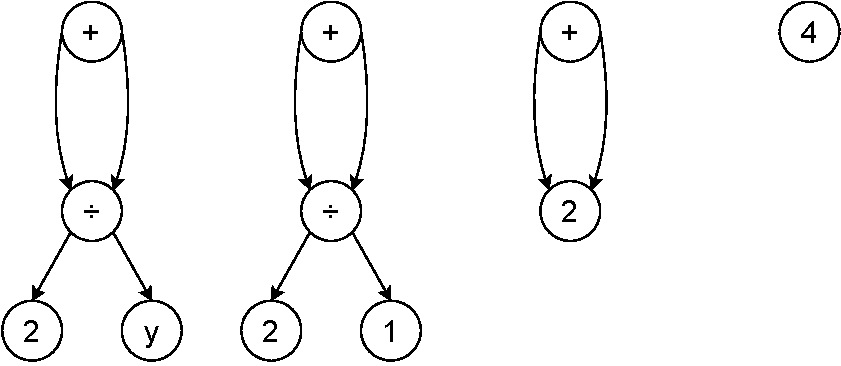
\includegraphics{graph-reduction}
  \caption[Schrittweise Reduktion eines Ausdrucks]{Schrittweise Redutkion des Ausdrucks $\mathtt{let}\ x\ =\ \frac{2}{y}\ \mathtt{in}\ x + x$}\label{fig:graph-reduction}
\end{figure}


\section{Besonderheiten der STG}

Die STG-Maschine definiert einige Erweiterungen für dieses Modell der Graphenreduktion.
Mit Hilfe dieser wird lazy Evaluation möglich und die effiziente Ausführung auf gewöhnlicher Hardware unterstützt.

Während die Darstellung eines Programms und dessen Ausdrücke als Knoten in einem Graph über die verschiedenen Ausprägungen der Laufzeitwerte abstrahiert und so im grundlegenden Modell die Unterscheidung zwischen Thunks, Werten und Closures für anonyme Funktionen überflüssig macht, müssen die durchgeführten Reduktionsregeln weiter eingeschränkt werden, um lazy Evaluation zu ermöglichen.
Dem Ansatz aus Abbildung~\ref{fig:graph-reduction} entsprechend würde der gesamte Graph reduziert, was der Idee der lazy Evaluation widerspricht.

Die Lösung ist hier das Definieren einer Normalform, welche die ausgewertete Form eines Ausdrucks darstellt.
Die Anwendung von Reduktionsregeln auf einen Teilgraphen in Normalform verändert diesen nicht mehr; ein Ende der Auswertung wurde erreicht.
Im Rahmen der \gls{stg} wird die \gls{whnf} verwendet~\cite{Wiki_Haskell}.
Die \gls{whnf} beschreibt, dass lediglich der Kopf eines Graphen in Normalform vorliegen muss, um ihn als ausgewertet zu betrachten.
Dies ist der Fall, wenn der oberste Knoten des Graphen einen Konstruktor oder eine eingebaute Funktionsanwendung beschreibt.
Der Rest des Graphen darf dabei unausgewertet vorliegen, wodurch die \gls{whnf} zu einer schwachen Normalform wird.
Am konkreten Beispiel einer verketteten Liste bedeutet dies, dass lediglich bekannt sein muss, ob der Kopf der Liste den Listenkonstruktor oder die leere Liste darstellt.
Ob die Liste abgesehen vom Kopf weitere Elemente enthält, wie lang diese Liste ist, oder wie das oberste Listenelement aussieht, ist dabei für die \gls{whnf} irrelevant.

Problematisch wird trotz der \gls{whnf} dennoch die Auswertung von unendlichen Graphen oder Graphen, die einen Zyklus enthalten.
Gerade endlose Graphen erweisen sich als Herausforderung, wenn man den naiven Ansatz verfolgt und den gesamten Programmgraphen als Datenstruktur im Speicher hat.
Diesen Problemfall behandelt das \textit{S} in \gls{stg}, welches für \textit{Spineless} steht.
Die sogenannte Spine bezeichnet dabei die Datenstruktur, welche im Hauptspeicher einer Maschine den Graphen enthält.
Bei der \gls{stg} existiert diese Datenstruktur nicht explizit.
Stattdessen werden Zeiger auf berechnete Werte oder Codeblöcke verwendet, die den Graphen repräsentieren.
Als Resultat wird während der Laufzeit nicht der gesamte Graph im Speicher gehalten, sondern nur der Teil, der für die aktuelle Auswertung relevant ist.

Die letzte Erweiterung der \gls{stg}, wird durch das \textit{T} beschrieben, welches für \textit{Tagless} steht.
Obwohl die Knoten im Modell der Graphenausführung Closures, Thunks und Werte vereinheitlichen, kann es nötig sein, während der Auswertung eines Ausdrucks, zwischen diesen Ausprägungen zu unterscheiden.
Ist der zu reduzierende Teil des Graphen ein Thunk, so muss die von diesem dargestellte unterbrochene Berechnung fortgesetzt werden.
Liegt ein bereits ausgewerteter Wert vor, so kann dieser direkt verwendet werden.

Die Unterscheidung der Ausprägungen geschieht in anderen Graphenmaschinen durch sogenannte Tags, welche einen Knoten markieren und dessen Ausprägung bestimmen \cn{Andere Maschinen?}.
Die \gls{stg} verwendet eine einheitliche Darstellung, in der alle Ausprägungen als Closure dargestellt werden.
Neben den freien Variablen, die sowohl bei herkömmlichen Closures als auch bei Thunks eingefangen und gespeichert werden müssen, enthält die einheitliche Darstellung einen Zeiger auf einen Codeblock anstelle eines Tags.
So wird es überflüssig, die korrekte Aktion zur Auswertung der Closure anhand des Tags zu bestimmen.
Der Zeiger verweist stattdessen auf den Code, der die gewünschte Aktion beschreibt und ein einfacher Sprung genügt, um diese auszuführen.
Closures können so Argumente vom Stack konsumieren und die Auswertung des Rumpfs beginnen, für Thunks wird die unterbrochene Ausführung angestoßen und für bereits ausgewertete Werte der jeweilige Wert zurückgegeben.

\begin{figure}[h]
  \centering
  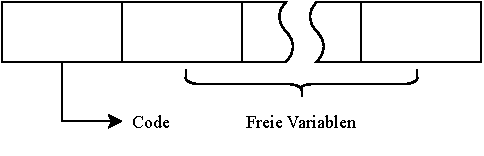
\includegraphics[width=0.8\textwidth]{closure-layout}
  \caption{Aufbau einer Closure}\label{fig:closure}
\end{figure}

%%% Local Variables:
%%% mode: latex
%%% TeX-master: "../Ausarbeitung"
%%% End:
